\documentclass{scrartcl}
\usepackage{german}
\usepackage[utf8]{inputenc}
\usepackage[german]{babel}

% zusätzliche mathematische Symbole, AMS=American Mathematical Society
\usepackage{amssymb}
\usepackage{amsmath}
% fürs Einbinden von Graphiken
\usepackage{graphicx}

% für Namen etc. in Kopf- oder Fußzeile
\usepackage{fancyhdr}

% erlaubt benutzerdefinierte Kopfzeilen
\pagestyle{fancy}

% used for drawing the gantt-diagram
\usepackage{pgfgantt}


% Definition der Kopfzeile
\lhead{
\begin{tabular}{lllll}
Nils Hagner & 4346038 & Felix Karg & 4342014 \\
Michael Fleig & 4340085 & Anush Davtyan &4368689
\end{tabular}
}
\chead{}
\rhead{\today{}}
\lfoot{}
\cfoot{Seite \thepage}
\rfoot{}

\begin{document}

\section*{Solutions for Excercise sheet 2}

\subsection*{Exercise 1 – Cost Estimation}
\begin{itemize}
	\item[i]
	The resulting amount should be $30h*6=180h$ per person, and with $1 PM=20*8=160h$ it amounts to $6.75$ PMs or with five persons to $5.625$ PMs.\\
	\item[ii]
	\begin{tabular} {| c | c |}
		round & estimations ($KLOC_{pars}$)\\
		\hline
		0 & 10, 15, 14, 15 \\
		1 & 12, 13, 12, 10\\
		2 & 12\\
	\end{tabular}\\\\
	Surprisingly, our estimates did not differ that much in the first round.
	By giving opinions for the lowest and the highest values, such as low experience leading to redundancy in the code, or that the use of a framework could reduce the amount of code, we came to the conclusion that the project should have about 12 $KLOC_{pars}$.
	\item[iii]
	We decided for small size, greater innovation, medium deadlines and stable development environment. Because of this we chose a medium project with $a=3.0$ and $b=1.12$.\\
	\item[iv]
		\item[]Required software reliability: nominal \\ If the system fails, the user can loose all points achieved in the game, but the points can be achieved again in not a very long time.
		\item[]Size of application database:  none \\
		It is very low, we do not need a database.
		\item[]Complexity of the product:  nominal \\
		It is nominal because: only standart math will be used; mostly simple nesting; some divice-dependent operations, like error prosessing, but barely operations at the physical I/O level; only simple structural changes and simple edits.
		\item[]Run-time performance constraints:   nominal \\
		Because the software is processor-intensive.
		\item[]Memory constraints:  nominal\\
		Because the group has only little experience, and we assume the program will be not very effective.
		\item[]Volatility of the virtual machine env.:  very low \\
		Because there are no changes of the working environment.
		\item[]Computer turnaround time:  low\\
		Because the game is (or should be) interactive.
		\item[]Analyst capability:  low\\
		Because of too little experience.
		\item[]Applications experience:  low \\
		Because the students do not have a lot of working experience.
		\item[]Software engineer capability:  nominal\\
		The developers should have some experience in teamwork.
		\item[]Virtual machine experience:  high \\
		Because the software(game) developing do not require very high virtual machine experience.
		\item[]Programming language experience:  very low\\
		Because the students have almost no experience in C\# or F\#.
		\item[]Use of modern programming practices:  low\\
		The group is only starting to use such practices.
		\item[]Use of software tools:  nominal\\
		Some useful software tools will be used, but since experience is missing it's unlikely to get fully utilized.
		\item[]Required development schedule:  nominal\\
		Because a fixed deadline is set.


	\item[v]
	\begin{tabular}{l | c}
		parameter & chosen value \\
		\hline

		Required software reliability & 1\\

		Size of application database & -\\

		Complexity of the product & 1\\

		Run-time performance constraints  & 1\\

		Memory constraints & 1\\

		Volatility of the virtual machine env. & -\\

		Computer turnaround time & 0.87\\

		Analyst capability & 1.19\\

		Applications experience & 1.13\\

		Software engineer capability & 1\\

		Virtual machine experience & 0.9\\

		Programming language experience & 1.14\\

		Use of modern programming practices & 1.1\\

		Use of software tools & 1\\

		Required development schedule & 1\\
	\end{tabular}\\\\
	The resulting project size in PM is (with $a=3$ and $b=1.12$):
	\[3 \cdot (12)^{1.12}\cdot (1\cdot 1 \cdot 1 \cdot 1 \cdot 0.87 \cdot 1.19 \cdot 1.13 \cdot 1 \cdot 0.9 \cdot 1.14 \cdot 1.1 \cdot 1 \cdot 1) \approx 64\]
	The two values differ drastically, the first is nearly a tenth of the second.
        This might be due to the way higher expectations of Code Quality or Project length, as well as the larger growth of smaller projects.
\end{itemize}

\subsection*{Exercise 2 – Process Modeling}

\begin{itemize}
    \item[i)] Process model: \\
        (Additionally: For the Specification there's a Requirenment Analyst responsible, as is a SW Developer for the Integrated System) \\
    	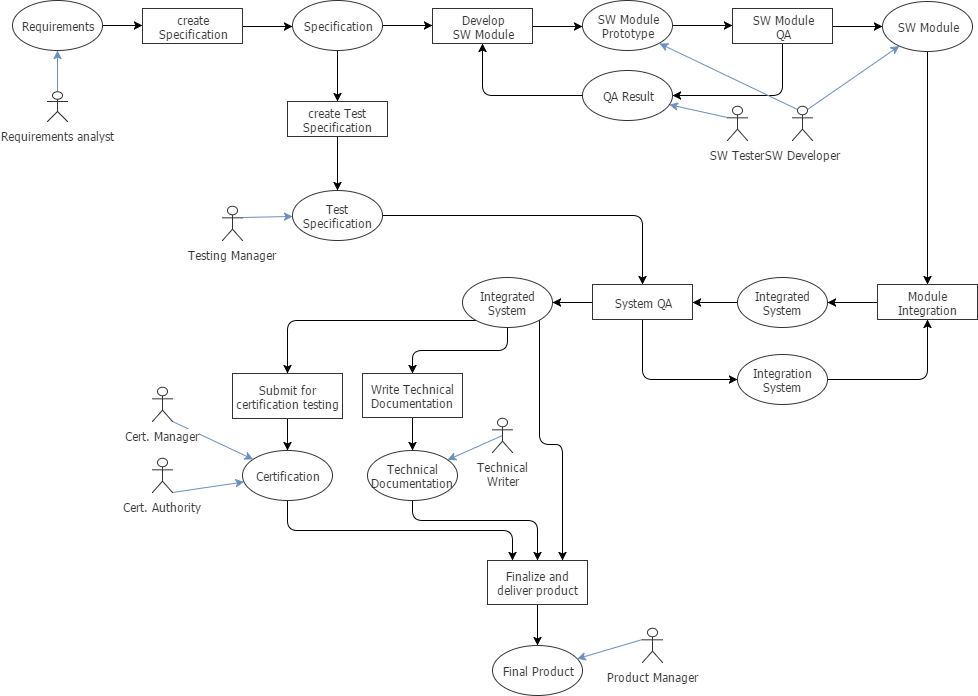
\includegraphics[width=\textwidth]{swt_2_1.png}
    \item[ii)]
        Tag 0: Project start. Requirenment Engineering start. \\
        Tag 12: Specification complete. Development of SW Module Prototype and Test Specification creation start. \\
        Tag 22: First Prototype of SW Module, SW Quality Assurance start \\
        Tag 25: SW QA finished, one Issue detected, start next cycle for SW Modules \\
        Tag 27: Issue fixed, Test specicfication finished, SW Modules now finished, Module Integration start \\
        Tag 40: Modules integrated, start testing using Test specification \\
        Tag 45: Modules fully integrated compliant to Test Spec, start of Certification Testing and writing of Technical documentation \\
        Tag 55: Certified and Documentation finished, Finialize Project. \\
    \item[iii)] (probably next page) \\
        % \documentclass{article}

% \usepackage{pgfgantt}

% \begin{document}


\begin{ganttchart}[
        hgrid,
        vgrid
    ]{1}{17}
    \gantttitle{Half Person-Months}{17} \\
    \gantttitlelist{1,...,17}{1} \\

    \ganttgroup{Maria}{1}{1}
    \ganttgroup{Maria}{11}{11} \\

    \ganttbar{Create Spec}{1}{1} \\

    \ganttgroup{Herbert}{2}{10} \\

    \ganttbar{SW Module Dev}{2}{4} \\
    \ganttbar{SW Module QA}{5}{6} \\
    \ganttbar{Module Integration}{7}{8} \\
    \ganttbar{System QA}{9}{10} \\
    \ganttbar{Create Test Spec}{11}{11} \\

    \ganttgroup{Karin}{12}{15} \\

    \ganttbar{Submit for cert Test}{12}{13} \\
    \ganttbar{Documentation}{14}{15} \\

    \ganttgroup{Jane}{16}{17} \\

    \ganttbar{Deliver}{16}{17}

\end{ganttchart} \\

I'm afraid to say that we were not capable of numbering through
correctly (in half PM's) or to correctly \LaTeX  quarter-PM's.
The used package seems to be not capable of doing so.

% \end{document}

    \item[iv)] Process model with fire detector \\
        (Additionally: For the Specification there's a Requirenment Analyst responsible, as is a SW Developer for the Integrated System) \\
    	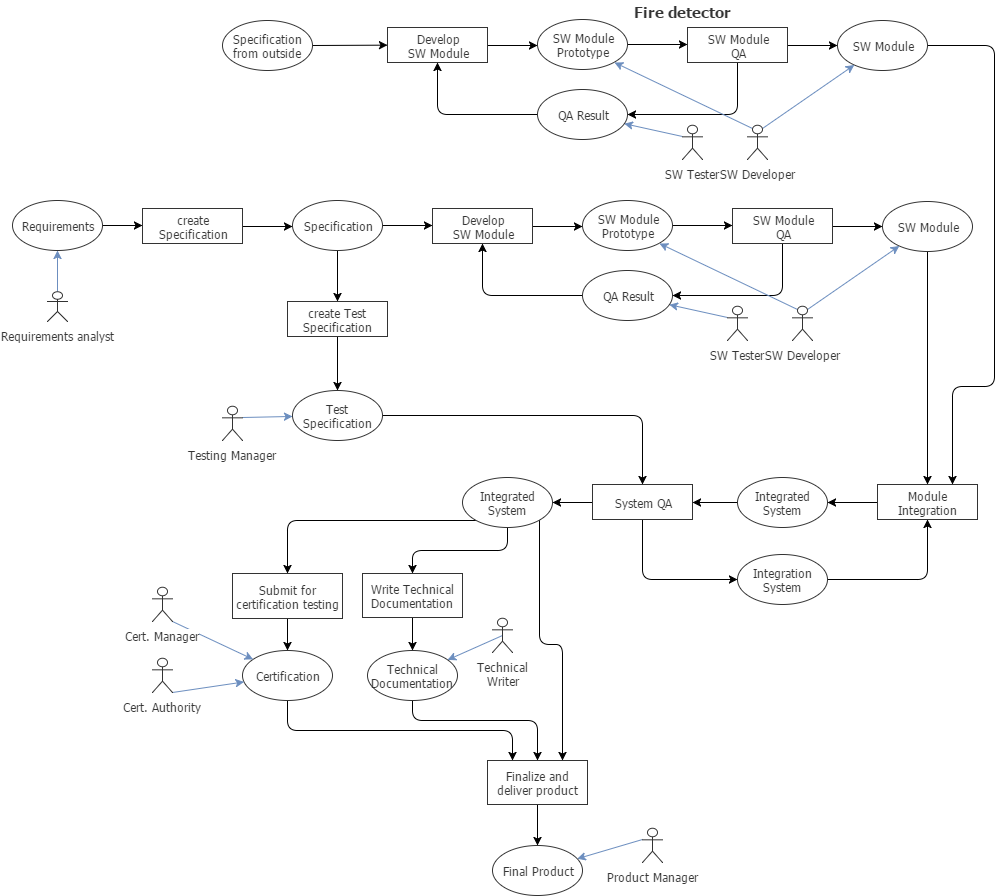
\includegraphics[width=\textwidth]{swt_2_3.png}
    \item[v)] Effort: 7.5 PM, minimum excpeted duration: 7.5 M
\end{itemize}

\end{document}
